\section{Estimación por intervalor}
\subsection{Introducción}
\begin{tcolorbox}[colback=blue!5!white, colframe=blue!75!black, title=\textbf{Estimación paramétrica}]
En el contecto e la estimación paramétrica, queremos aprovechar nuestro conocimiento sobre la distribución muestral de estimador, para proporcionar margen de error y riesgo.
\end{tcolorbox}
\begin{tcolorbox}[colback=blue!5!white, colframe=blue!75!black, title=\textbf{Bootstrap}]
También construiremos intervalos de confianza basados en percentiles Bootstrap.
\end{tcolorbox}
\begin{tcolorbox}[colback=red!5!white, colframe=red!75!black, title=\textbf{Idea básica}]
Supongamos:
\begin{itemize}[label=\textbullet]
    \item $X\sim \mathcal{N}(\mu,4)$.
    \item Consideramos una muestra aleatoria simple $X_1,\dots,X_4$, estimamos $\mu$ con $\overline{X}$.
\end{itemize}
Deducimos:
\begin{itemize}[label=\textbullet]
    \item Sabemos que $\overline{X}\sim \mathcal{N}(\mu,1)$.
    \item Implica: el 95\% de los valores de $\overline{X}$ está aproximadamente entre $\mu\pm 2$.
    \item Si sé dónde está $\mu$, sé que, con probabilidad 0.95, $\overline{X}$ se encuentre a menos de 2 unidades.
    \item Ahora al revés: si he observado un valor de $\overline{X}$, ¿dónde está $\mu$? la probabilidad de que $\mu$ se encuentre a menos de 2 unidades de $\overline{X}$ es 0.95.
\end{itemize}
\end{tcolorbox}
La probabilidad de que, habiendo observado un valor de $\overline{X},\mu$ se encuentre a menos de 2 unidades es $0.95$.
 \[
\mu\in \overline{X}\pm 2,\quad \text{con probabilidad 0.95}
\] 
\begin{itemize}[label=\textbullet]
    \item $\overline{X}\pm 2$ es un intervalo aleatorio.
    \item Para una muestra concreta que extraigamos, será $\overline{x}\pm 2$.
    \item $\pm 2$ expresa el margen de error.
    \item "con probabilidad 0.95" expresa la confianza que tenemos en que nuestra información sea cierta.
    \item Corremos un riesgo de error de 0.05 al afirmar,  $\mu\in \overline{X}\pm 2$.
\end{itemize}
\begin{tcolorbox}[colback=blue!5!white, colframe=blue!75!black, title=\textbf{Definición}]
\begin{itemize}[label=\textbullet]
    \item $(X_1,\dots,X_n)$ una muestra asociada a $f_\theta$.
    \item Un \lb{intervalo de estimación} está asociado por dos estadísticos $I(X_1,\dots,X_n)$ (extremo inferior) y $D(X_1,\dots,X_n)$ (extremos superior) y persigue capturar el valor del parámetro $\theta$.
\end{itemize}
\end{tcolorbox}
\begin{tcolorbox}[colback=red!5!white, colframe=red!75!black, title=\textbf{Un intervalo de estimación es aleatorio}]
\begin{itemize}[label=\textbullet]
    \item Sus extremos dependen de la muestra concreta escogida.
    \item $\theta \in [I(X_1,\dots,X_n),D(X_1,\dots,X_n)]$ define un suceso aleatorio.
    \item La probabilidad de este suceso $\mathbb{P}_\theta[\theta\in [I(X_1,\dots,X_n),D(X_1,\dots,X_n)]]$ se llama \textbf{nivel de cobertura} del intervalo para este valor de $\theta$.
    \item El nivel de cobertura depende de $\theta$.
\end{itemize}
\end{tcolorbox}
\subsection{Nivel de confianza}
\begin{itemize}[label=\color{red}\textbullet, leftmargin=*]
    \item \lb{Nivel de cobertura} \[
            \theta\longmapsto \mathbb{P}_\theta[\theta\in [I(X_1,\dots,X_n),D(X_1,\dots,X_n)]]]
    \] 
    El \lb{nivel de confianza} es el valor mínimo del nivel de cobertura calculado cuando varía $\theta$. 
\end{itemize}
\begin{tcolorbox}[colback=olive!5!white, colframe=olive!75!black, title=\textbf{Confianza vs Precisión}]
Deberemos buscar una alta confianza pero sin sacrificar en exceso la precisión.
\end{tcolorbox}
\subsection{Un procedimiento general de construcción}
Se aplica en muchas situaciones de modelización.
\begin{tcolorbox}[colback=blue!5!white, colframe=blue!75!black, title=\textbf{Procedimiento}]
\begin{itemize}[label=\textbullet]
    \item Nos fijamos el "nivel de riesgo", $0<\alpha<1$, por ejemplo, $0.1,0.05$, o  $0.01$.
    \item Buscamos  $T(X_1,\dots,X_n)$ que se \lb{pivotal}, es decir, que su distribución no depende de $\theta$.
    \item Escogemos dos cotas $a$ y  $b$:  \[
            \mathbb{P}_\theta[a\le T(X_1,\dots,X_n)\le b]=1-\alpha,\quad \forall \theta\in \Theta.
    \] 
\item Procuramos despejar $\theta$: \[
        \mathbb{P}_\theta[I(X_1,\dots,X_n)\le \theta\le D(X_1,\dots,X_n)]=1-\alpha.
\] 
\end{itemize}
\end{tcolorbox}
\begin{tcolorbox}[colback=red!5!white, colframe=red!75!black, title=\textbf{Nota}]
\begin{itemize}[label=\textbullet]
    \item $T$ es pivotal $\longrightarrow $ el nivel de cobertura $1-\alpha$ de $[I(X_1,\dots,X_n),D(X_1,\dots,X_n)]$ no depende de $\theta$.
    \item $1-\alpha$ es el nivel de confianza.
\end{itemize}
\end{tcolorbox}
\subsection{Intervalo de confianza para la media $\mu$ de $X\sim \mathcal{N}(\mu,\sigma^2),\sigma$ conocida}

\lb{Consideramos una muestra aleatoria simple de una distribución $X\sim \mathcal{N}(\mu,\sigma^2)$. El valor de $\sigma^2$ es conocido}
\begin{itemize}[label=\textbullet]
    \item Usaremos $\overline{X}$ para estimar $\mu$.
\end{itemize}
Estadístico pivotal: \[
    T(X_1,\dots,X_n;\theta)=\dfrac{\overline{X}-\mu}{\sigma / \sqrt{n} }\sim \mathcal{N}(0,1).
\] 
\begin{itemize}[label=\textbullet]
    \item Dibujamos en la densidad del estadístico pivotal $\dfrac{\overline{X}-\mu}{\sigma / \sqrt{n} }$, una región central que represente el $100(1-\alpha)\%$ del área total.
\end{itemize}
\begin{center}
    \includegraphics[width=0.5\textwidth]{"Tema 3/figures/Figure 1"}
\end{center}
\begin{tcolorbox}[colback=olive!5!white, colframe=olive!75!black, title=\textbf{Cuantil}]
Para $0\le u\le 1, z_u$ es el \textbf{cuantil} $u$ de una $\mathcal{N}(0,1)$, es decir, el valor que cumple $\mathbb{P}(Z\le z_u)=u$.
\end{tcolorbox}
\[
\mathbb{P}\left[ -z_{1-\alpha /2}\le \dfrac{\overline{X}-\mu}{\sigma / \sqrt{n} }\le z_{1-\alpha /2} \right] =1-\alpha.
\] 
Despejamos $\mu$:
\begin{itemize}[label=\textbullet]
    \item $\mathbb{P}\left[ \overline{X}-z_{1-\alpha / 2}\dfrac{\sigma}{\sqrt{n} }\le \mu\le \overline{X}+z_{1-\alpha /2}\dfrac{\sigma}{\sqrt{n} } \right] =1-\alpha$
    \item El \lb{intervalo de confianza} al $100(1-\alpha)\%$ para $\mu$ es: \[
    \mu\in \left( \overline{X}-z_{1-\alpha / 2}\dfrac{\sigma}{\sqrt{n} };\overline{X}+z_{1-\alpha / 2}\dfrac{\sigma}{\sqrt{n} } \right) .
    \] 
\item De forma equivalente: $\mu\in \overline{X}\pm z_{1-\alpha / 2}\dfrac{\sigma}{\sqrt{n} }.$
\end{itemize}
\begin{tcolorbox}[colback=olive!5!white, colframe=olive!75!black, title=\textbf{Margen de error}]
$z_{1-\alpha /2}\dfrac{\sigma}{\sqrt{n} }$ se llama \textbf{término de error}. 
\end{tcolorbox}
\subsubsection{Interpretación}
\begin{tcolorbox}[colback=red!5!white, colframe=red!75!black, title=\textbf{Importante}]
\begin{itemize}[label=\textbullet]
    \item El intervalo de confianza $\left[ \overline{X}-z_{1-\alpha /2}\dfrac{\sigma}{\sqrt{n} };\overline{X}+z_{1-\alpha /2}\dfrac{\sigma}{\sqrt{n} } \right] $ es un intervalo \textbf{aleatorio}.
    \item Al extraer una muestra, tengo una probabilidad $\alpha$ de que, al afirmar que $\mu$ se encuentra en $\left[ \overline{X}-z_{1-\alpha / 2}\dfrac{\sigma}{\sqrt{n} };\overline{X}-z_{1-\alpha /2}\dfrac{\sigma}{\sqrt{n} } \right] $, me equivoque.
\end{itemize}
\end{tcolorbox}
\begin{center}
    \includegraphics[width=0.7\textwidth]{"Tema 3/figures/Figure 2"}
\end{center}

\lb{\underline{Ejemplo:} } 

\begin{itemize}[label=\textbullet]
    \item Queremos estimar la longitud media de un artículo producido por una máquina.
    \item Por experiencia, sabemos que es razonable modelizar la distribución de los valores de la longitud de los artículos producidos por una distribución Normal con media $\mu$ y desviación típica a 0.05.
    \item Para estimar $\mu$ extraemos una muestra de 5 artículos: \[
    20.1,20.05,19.95,19.99.
    \]
\item Construir un intervalo de confianza al 90\%.
\end{itemize}
\begin{minipage}{0.45\textwidth}
    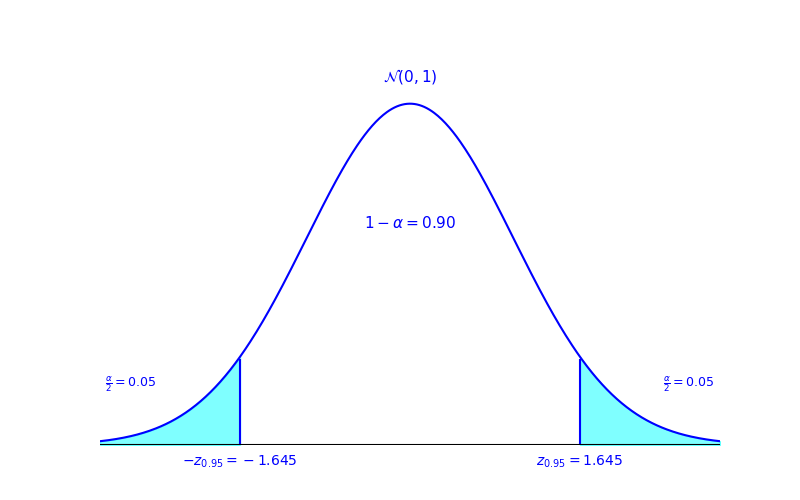
\includegraphics[width=\linewidth]{Tema 3/figures/Figure 3}
\end{minipage}
$\begin{array}{l}
    \overline{x}=20.02\\
1-\alpha=0.09\\
\alpha=0.1\\
\dfrac{\alpha}{2}=0.05\\
\left(20.2\mp 1.645 \dfrac{0.05}{\sqrt{5} }\right)=(20.02\mp 0.0367) = (19.9833, 20.0588)
\end{array}$

\subsection{Comentarios importantes}
\begin{tcolorbox}[colback=olive!5!white, colframe=olive!75!black, title=\textbf{Si $X$ no es Normal}]
\begin{itemize}[label=\textbullet]
    \item Hemos trabajado con la hipótesis de que $X$ es Normal para encontrar el estadístico pivotal $\dfrac{\overline{X}-\mu}{\sigma / \sqrt{n} }\sim \mathcal{N}(0,1)$.
    \item Si $X$ no es Normal, no podemos garantizar la confianza especificada.
    \item Sin embargo, si $n$ grande, tenemos por el Teorema Central del Límite \[
    \dfrac{\overline{X}-\mu}{\sigma / \sqrt{n} }\sim \mathcal{N}(0,1),\text{ aproximiadamente, }
    \] 
    entonces la confianza especificada no será exacta pero casi\dots
\end{itemize}
\end{tcolorbox}
\subsubsection{Factores que afectan a la precisión de la estimación}
\begin{tcolorbox}[colback=olive!5!white, colframe=olive!75!black, title=\textbf{El margen de error es $z_{1-\alpha /2}\dfrac{\sigma}{\sqrt{n} }$.}]
\begin{itemize}[label=\textbullet]
    \item $n\uparrow\longrightarrow \text{ precisión }\uparrow$
    \item $\sigma\uparrow\longrightarrow \text{ precisión }\downarrow$ 
    \item Confianza $\uparrow\longrightarrow $ precisión $\downarrow$
\end{itemize}
\end{tcolorbox}
\subsubsection{Determinación del tamaño muestral}
\begin{tcolorbox}[colback=blue!5!white, colframe=blue!75!black, title=\textbf{Contexto}]
Antes de extraer la muestra:
\begin{itemize}[label=\textbullet]
    \item Tenemos decidido el valor de $\sigma$.
    \item Tenemos decidido la confianza con la que trabajamos.
    \item Tenemos decidio el margen de error máximo $max$ que estamos dispuestos a comenter.
\end{itemize}
¿Qué tamaño de la muestra debemos escoger?
\end{tcolorbox}
Margen de error: $z_{1-\alpha /2}\dfrac{\sigma}{\sqrt{n} }\le max.\longrightarrow $ Despejamos $n$
\subsubsection{Otros modelos, estadísticos pivotales}
 \begin{tcolorbox}[colback=blue!5!white, colframe=blue!75!black, title=\textbf{$X\sim \mathcal{N}(\mu,\sigma^2)$, estimamos $\mu,\sigma$ desconocida}]
Estadístico pivotal: \[
T=\dfrac{\overline{X}-\mu}{S / \sqrt{n} }\sim t_{n-1}
\] 
\end{tcolorbox}

Debemos encontrar valores $a$ y $b$ tales que:

\begin{minipage}{0.45\textwidth}
    \includegraphics[width=\linewidth]{"Tema 3/figures/Figure 4"}
\end{minipage}$\begin{array}{l}
    P\left[ a\le \dfrac{\overline{X}-\mu}{S / \sqrt{n} }\le b \right] \\
    P\left[ -t_{n-1,1-\frac{\alpha}{2}}\le \dfrac{\overline{X}-\mu}{S / \sqrt{n} }\le t_{n-1,1-\frac{\alpha}{2} } \right] \\
    P\left[ X-t_{n-1,1-\frac{\alpha}{2} }\dfrac{S}{\sqrt{n} }\le \dfrac{\overline{X}-\mu}{S / \sqrt{n} }\le X+t_{n-1,1-\frac{\alpha}{2} }\dfrac{S}{\sqrt{n} } \right] =1-\alpha
\end{array}$

Obteniendo como I.C aleatorio a nivel $100(1-\alpha)\%$ \[
X-t_{n-1,1-\frac{\alpha}{2} }\dfrac{S}{\sqrt{n} }
\] 
\begin{tcolorbox}[colback=blue!5!white, colframe=blue!75!black, title=\textbf{$X\sim \mathcal{N}(\mu,\sigma^2)$, estimamos $\sigma^2$}]
Estadístico pivotal: \[
\dfrac{(n-1)S_n^2}{\sigma^2}\sim \chi_{n-1}^2
\] 
\end{tcolorbox}
I.C para $\sigma^2$ al nivel de confianza $(1-\alpha)100\%$ \[
T=\dfrac{(n-1)s^2}{\sigma^2}\leadsto \chi_{n-1}^2
\] 
Debemos encontrar valores $a$ y $b$ tales que: $P\left[ a\le \dfrac{(n-1)s^2}{\sigma^2}\le b \right]=1-\alpha $

\begin{minipage}{0.45\textwidth}
    \includegraphics[width=\linewidth]{"Tema 3/figures/Figure 5"}
\end{minipage}
$\begin{array}{l}
    P\left[ -\chi_{n-1,\frac{1-\alpha}{2} }^2\le \dfrac{(n-1)s^2}{\sigma^2}\le \chi_{n-1,1-\frac{\alpha}{2} }^2 \right] =1-\alpha\\
    P\left[ -\dfrac{1}{\chi_{n-1,1-\frac{\alpha}{2}}} \le  \dfrac{\sigma^2}{(n-1)s^2}\le \dfrac{1}{\chi_{n-1,1-\frac{\alpha}{2} }^2} \right] =1-\alpha\\
    P\left[ -\dfrac{(n-1)s^2}{\chi_{n-1,1-\frac{\alpha}{2} }^2}\le \sigma^2\le \dfrac{(n-1)s^2}{\chi_{n-1,1-\frac{\alpha}{2} }^2} \right] =1-\alpha
\end{array}$
